\documentclass{llncs}


\usepackage{hyperref}
\usepackage{graphicx}
\usepackage{multirow}
\usepackage[misc,geometry]{ifsym}

\usepackage{amsmath}
\usepackage{enumitem}
%\usepackage{amsfonts}
%\usepackage{amssymb}
%\usepackage{epstopdf}
%\usepackage{epsfig}

\usepackage[utf8x]{inputenc}
\usepackage[english,russian]{babel}



\begin{document}

\mainmatter 

\title{Parallel Global Optimization for Non-Convex Mixed-Integer Problems
\thanks{This study was supported by the Russian Science Foundation, 
project No.\,16-11-10150.}}
\author{Konstantin Barkalov \and Ilya Lebedev %\Letter 
\\
\email{konstantin.barkalov@itmm.unn.ru}}

\institute{
Lobachevsky State University of Nizhni Novgorod, Nizhni Novgorod, Russia
}

\maketitle

\begin{abstract}
In the present paper, the mixed-integer global optimization problems are considered. A novel 
deterministic algorithm for solving the problems of this class based on the information-statistical 
approach to solving the continuous global optimization problems has been proposed. The 
comparison of this algorithm with known analogs demonstrating the efficiency of the 
developed approach has been conducted. The stable operation of the algorithm was confirmed 
also by solving a series of several hundred mixed-integer global optimization problems. 

\keywords global optimization, non-convex constraints, mixed-integer problems.

\end{abstract}

\section{Introduction}\label{sec:intro}

In the present paper, the global optimization problems and the method of solving these ones are 
considered. The global optimization problems are the computation-costly ones since the global 
optimum is an integral characteristic of the problem being solved and requires the investigation 
of the whole search domain. 
%As a result, the search of the global optimum is reduced to the construction of a coverage (in general, a nonuniform one) of the space of parameters. 
The problems, in which some parameters can take the integer values only (mixed-integer global 
optimization problems) are of special interest because for these ones it is more difficult to build 
the estimates of the optimum as compared to the continuous problems.

A lot of publication have been devoted to the methods of solving the mixed-integer problems 
(see, for example, the reviews~\cite{Burer,Boukouvala}). The well known deterministic 
methods of solving the problems of this class are based, as a rule, on the Branch-and-Bound 
approach or on the Branch-and-Reduce one. Also, a number of the metaheuristic and genetic 
algorithms are known, which are based one way or another on the random search concept.
%  based ones, anyway, based on the ideas of random search.

In the present study, we proposed a novel deterministic method for solving the mixed-integer 
problems based on the information-statistical approach to solving the global optimization 
problems \cite{Strongin2000,Strongin2013}. The paper text reflecting the results of preliminary 
studies is composed as follows. First, an approach to solving the problems with continuous 
parameters has been considered, then its generalization for the mixed-integer problems was 
proposed. In the final section, the results of comparison of the proposed method with the 
known analogs are presented.

\section{Global optimization algorithm and dimension reduction}

A constrained global optimization problem can be formulated as follows
%Let us consider the $N$-dimensional global optimization problem
\begin{gather}\label{problem}
\varphi(y^\ast)=\min{\left\{\varphi(y):y\in D, \; g_i(y)\leq 0, \; 1 \leq i \leq m\right\}},\\
D=\left\{y\in R^N: a_j\leq y_j \leq b_j, 1\leq j \leq N \right\}.\label{D}
\end{gather}
The objective function $\varphi(y)$ (hereafter denoted by $g_{m+1}(y)$) and the left-hand 
sides $g_i(y), \; 1\leq i \leq m,$ of the constraints satisfy the Lipschitz condition 
\[
\left|g_i(y_1)-g_i(y_2)\right|\leq L_i\left\|y_1-y_2\right\|, \;1\leq i\leq m+1, \; y_1,y_2 \in D,\;
\]
with a priori unknown constants $L_i, \; 1 \leq i \leq m+1,$ and may be multiextremal. It is 
assumed that the functions $g_i(y)$ are defined and computable only at the points $y \in D$ 
satisfying the conditions
\begin{equation}\label{g_k}
g_k(y) \leq 0, \; 1 \leq k < i.
\end{equation}

By employing the continuous single-valued Peano-Hilbert curve $y(x)$ mapping the unit interval 
$[0,1]$ on the $x$-axis onto the $N$-dimensional domain (\ref{D}), it is possible to find the 
minimum in (\ref{problem}) by solving the one-dimensional problem
\[
\varphi(y(x^\ast))=\min \left\{\varphi(y(x)): x \in [0,1], \; g_i(y(x))\leq 0, \; 1 \leq i \leq m\right\}.
\]
Algorithms for numerical construction of Hilbert curve approximation (\textit{evolvent}) are 
considered in \cite{Strongin2013}. These evolvents are fractals generated by an iterative
process, that fill in the hypercube $D$ with accuracy $2^{-m}$, where integer $m>0$ is the evolvent construction parameter. 
%Пример разверток - рисунки: 2D или 3D?
%Examples of the evolvent with different m in two dimensions are given in Fig. 1.
%In Fig. 1 approximations of levels 1, 2, 3, and 4 of the Hilbert curve are given in the domain [􀀀1; 1] \in R3.


Due to (\ref{g_k}) the functions $g_i(y(x))$ are defined 
and computable in the subranges 
\[
Q_1=[0,1], \; Q_{i+1}=\left\{x \in Q_i : g_i(y(x)) \leq 0 \right\}, \; 1 \leq i \leq m.
\]

These conditions allows us to introduce a classification of the points $x \in [0,1]$ according to 
the number $\nu (x)$ of the constraints computed at this point. The \textit{index} $\nu(x)$ can 
also be defined by the conditions
\begin{equation}\label{nu}
g_i(y(x)) \leq 0, \; 1 \leq i < \nu, \; g_\nu(y(x))>0,
\end{equation}
where the last inequality is inessential if $\nu=m+1$.

In the dimensionality reduction scheme considered here, a multidimensional problem with 
Lipschitzian functions is juxtaposed with a one-dimensional problem, where the corresponding 
functions satisfy uniform H{\"o}lder condition (see \cite{Strongin2013}), i.e.,
\[
\left|g_i(y(x_1))-g_i (y(x_2))\right| \leq H_i \left|x_1-x_2 \right|^{1/N}, \; x_1,x_2\in [0,1], \; 
1\leq i \leq m+1.
\]
Here, $N$ is the dimensionality of the initial multidimensional problem and the coefficients 
$H_i$ are related to the Lipschitz constant $L_i$ of the initial problem as $H_i \leq 2L_i 
\sqrt{N+3}$.

Thus, \textit{a trial} at a point $x^k \in [0,1]$ executed at the $k$-th iteration of the algorithm 
will consist of the following sequence of operations:
\begin{itemize}
	\item Determine the \textit{image} $y^k=y(x^k)$ in accordance with the mapping 
$y(x)$;
	\item Compute the values $g_1(y^k),..., g_\nu(y^k),$ where $\nu = \nu(x^k)$ is from 
(\ref{nu}). 
\end{itemize}
The dyad 
\begin{equation} \label{trial_result}
 \{ \nu=\nu(x^k), \; z^k=g_\nu(y(x^k)) \} 
\end{equation}
will be referred to as the \textit{trial outcome}.

An efficient parallel index algorithm (PIA) for solving the constrained global optimization problem (\ref{problem}) has been developed at University of Nizhni Novgorod. 

Suppose we have $p \geq 1$  computational elements (e.g., accelerator cores), which can be used to run $p$ trials simultaneously. In the first iteration of the method, $p$ trials are run in parallel at various random points $x^i\in(0,1)$, $1\leq i \leq p$. 
Suppose $n \geq 1$  iterations of the method have been completed, and as a result of which, trials were carried out in $k=k(n)$ points $x^i, 1\leq i \leq k$. Then the points $x^{k+1},...,x^{k+p}$  of the search trials in the next $(n+1)$-th iteration will be determined according to the rules below.

\begin{enumerate}
\item 
Renumber the points $x^1,...,x^k$ from previous iterations with lower indices, lowest to highest coordinate values, i.e.
\begin{equation}\label{Eq:17}
0=x_0<x_1<...<x_i<...<x_k<x_{k+1}=1,
\end{equation}
and match them with the values $z_i=g_\nu(y(x_i))$, $\nu=\nu(x_i)$, $1 \leq i \leq k$, from (\ref{trial_result}), calculated at these points; points $x_0=0$ и $x_{k+1}=1$ are introduced additionally; the values $z_0$ и $z_{k+1}$ are indeterminate.
\item
Classify the numbers $i,1\leq i \leq k$, of the trial points from (\ref{Eq:17}) by the number of problem constraints fulfilled at these points, by building the sets
\begin{equation}\label{Eq:18}
I_\nu = \left\{i: 1 \leq i \leq k,\ \nu = \nu(x_i)\right\},\ 1 \leq \nu \leq m+1,
\end{equation}
containing the numbers of all points $x_i,1\leq i \leq k$, with the same values of $\nu$. The end points $x_0=0$ and $x_{k+1}=1$ are interpreted as those with zero indices, and they are matched to an additional set $I_0={0,k+1}$. 

Identify the maximum current value of the index
\begin{equation}\label{Eq:19}
M=\max \left\{\nu = \nu(x_i), \ 1\leq i \leq k\right\}.
\end{equation}
\item
For all values of $\nu, \ 1\leq \nu \leq m+1$, calculate the values  
\begin{equation}\label{Eq:20}
\mu_\nu = \max \left\{ \frac{\left|z_i-z_j\right|}{\left(x_i-x_j\right)^{1/N}} : i,j \in I_\nu, j<i\right\}.
\end{equation}
If the set $I_\nu$ contains less than two elements or $\mu_\nu$ from (\ref{Eq:20}) equals zero, then assume $\mu_\nu=1$.
\item
For all non-empty sets $I_\nu$, $1 \leq \nu \leq m+1$, determine the values
\begin{equation}\label{Eq:21}
  z^\ast_\nu =  
   \begin{cases}
    -\epsilon_\nu,  \nu < M, \\
    \min{\left\{g_\nu(x_i):i\in I_\nu\right\}}, \nu = M,
   \end{cases}
\end{equation}
where $M$ is the maximum current value of the index, and the vector
\begin{equation}\label{Eq:22}
\epsilon _R=\left(\epsilon_1,...,\epsilon_m\right),
\end{equation}
with positive coordinates is called the \textit{reserve vector} and is used as a parameter in the algorithm.
\item
For each interval $(x_{i-1},x_i)$,$1 \leq i \leq k+1$, calculate the \textit{characteristic} $R(i)$: 
\[
R(i)=\Delta_i+ \frac{(z_i-z_{i-1})^2}{(r_\nu\mu_\nu)^2\Delta_i}-2\frac{z_i+z_{i-1}-2z^\ast_\nu}{r_\nu\mu_\nu},\;\; \nu=\nu(x_{i-1})=\nu(x_i),
\]
\[
R(i)= 2\Delta_i-4\frac{z_i-z^\ast_\nu}{r_\nu\mu_\nu},\;\; \nu(x_{i-1})<\nu(x_i)=\nu,
\]
\[
R(i)= 2\Delta_i-4\frac{z_{i-1}-z^\ast_\nu}{r_\nu\mu_\nu},\;\; \nu = \nu(x_{i-1})>\nu(x_i).
\]
where $\Delta_i=(x_i-x_{i-1})^{1/N}$, and the values $r_\nu>1, 1\leq\nu\leq m+1$, are used as parameters in the algorithm.
\item
Reorder the characteristics $R(i)$, $1\leq i \leq k+1$, from highest to lowest 	
\begin{equation}\label{Eq:23}
R(t_1)\geq R(t_2)\geq ... \geq R(t_{k})\geq R(t_{k+1})
\end{equation}
and choose $p$ largest characteristics with interval numbers $t_j, 1\leq j \leq p$.
\item
Carry out $p$ new trials in parallel at the points $x^{k+j}, 1 \leq j \leq p$, calculated by the formulae
\begin{eqnarray*}
& x^{k+j}=\frac{x_{t_j}+x_{t_j-1}}{2}, \; \nu(x_{t_j-1})\neq \nu(x_{t_j}), \\
& x^{k+j}=\frac{x_{t_j}+x_{t_j-1}}{2}- \frac{\mathrm{sign}(z_{t_j}-z_{t_j-1})}{2r_\nu}\left[\frac{\left|z_{t_j}-z_{t_j-1}\right|}{\mu_\nu}\right]^N, \; \nu(x_{t_j-1})=\nu(x_{t_j})=\nu. \\
\end{eqnarray*} 

%Добавить результаты испытаний в информационную базу алгоритма, и перейти к правилу 1.
\end{enumerate}

The algorithm stops if the condition $\Delta_{t_j}\leq \epsilon$ becomes true for at least one number $t_j, 1\leq j \leq p$; here  $\epsilon>0$ has an order of magnitude of the desired coordinate accuracy.

A detailed description of the algorithm convergence theory is presented in \cite{Strongin2000}.

\section{Parallel algorithm for mixed-integer problems}

Рассмотрим теперь случай, когда аргумент функций задачи содержит две компоненты: вектор $y$, принадлежащий гиперинтервалу $D$, и вектор $u$, имеющий конечный (и при этом не очень большой) набор возможных значений, т.е. 
\begin{gather}\label{problem_i}
\min{\left\{ g_{m+1}(y,u):y\in D, \; g_i(y,u)\leq 0, \; 1 \leq i \leq m\right\}},\\
D=\left\{a_j\leq y_j \leq b_j, \; 1\leq j \leq N \right\}.\nonumber
\end{gather}

Такие конечные наборы могут характеризовать, например, вариант материала, из которого создается объект, геометрические размеры или другие величины, которые могут принадлежать стандартному дискретному ряду, и т.п.

Занумеруем целыми числами $s, 1\leq s \leq S,$ все возможные значения вектора $u$, т.е. сопоставим каждому рассматриваемому значению $s$ вектор $u_s$. 
Тогда рассматриваемая задача может быть записана в виде 
\begin{gather}\label{problem_is}
 \min_{s\in\{1,...,S\}}\left(\min{\left\{ g_{m+1}(y,u_s):y\in D, \; g_i(y,u_s)\leq 0, \; 1 \leq i \leq m\right\}}\right),\\
D=\left\{ a_j\leq y_j \leq b_j, \; 1 \leq j\leq N \right\}.\nonumber 
\end{gather}

Используя схему редукции размерности с помощью развертки $y(x), x\in [0,1]$ можно сопоставить каждой вложенной задаче минимизации по $y$ одномерную задачу минимизации
\[
 \min{\left\{ g_{m+1}(y(x),u_s):x \in [0,1], \; g_i(y(x),u_s)\leq 0, \; 1 \leq i \leq m\right\}}, s\in\{1,...,S\}.
\]

Рассмотрим теперь соответствие 
\[
Y(x)=y(x-E(x)), \; x\in[0,S],
\]
отображающее любую точку интервала [0,S] на область $D$ (обозначение $E(x)$ соответствует целой части числа $x$) и определим функции 
\[
g_i(x) = g_i(Y(x),u_{E(x)+1}), x\in[0,S],
\]
имеющие, вообще говоря, разрывы первого рода в целочисленных точках $x_k = i, 1\leq i \leq S-1$.
%значения функций и индексов в данных точках - не определены!
Используя введенные обозначения можно переформулировать исходную задачу как
\begin{equation}\label{problem_is1}
\min \left\{g_{m+1}(x): x \in [0,S], \; g_i(x) \leq 0, \; 1 \leq i \leq m\right\}.
\end{equation}




As an illustration, Fig. \ref{fig:1} presents the plots of the functions corresponding to a 
problem with one continuous parameter and one binary parameter.

\begin{figure}[ht]
    \centering
    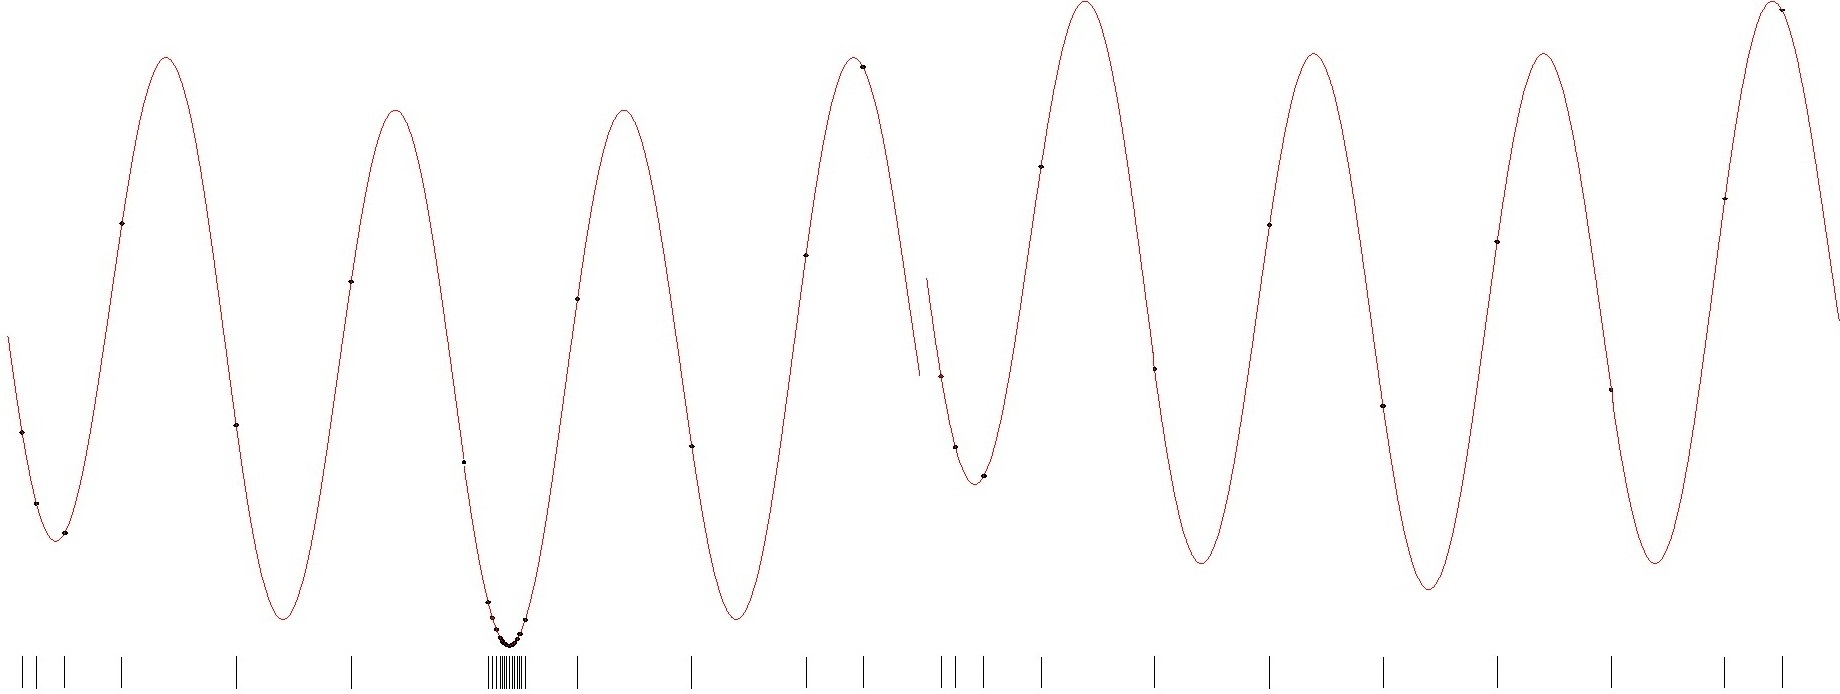
\includegraphics[width=1.0\textwidth] {fig1.jpg}
    \caption{Reduced mixed-integer global optimization problem}
    \label{fig:1}
\end{figure}

Applying the parallel index algorithm to solving the problem (\ref{problem_is1}), we will find 
the solution of the problem (\ref{problem_i}). In this case the major part of trials will conducted in 
the subproblem, the solving of which corresponds to the solving of the initial 
problem (\ref{problem_i}). In the rest subproblems, a only minor part of trials will be performed 
since the solutions of these subproblems are the locally optimal ones.
%with respect to the solution of the $s$-th subproblem. 
All the above is confirmed by Fig. \ref{fig:1}, where the  
points of trials executed in the course of solving this problem are denoted by the dashes.


Thus, we have constructed the \textit{Mixed-Integer Parallel Index Algorithm} (MIPIA) based on the  
reduction of the mixed-integer non-convex optimization problem to the non-convex optimization problem. 
%It is possible to prove that the convergence conditions for this algorithm will follow from the convergence conditions of its prototype (GSA).

Наиболее эффективно на GPU можно реализовать операцию вычисления сразу многих значений целевой функции. Для этого требуется реализовать на GPU процедуру вычисления значений функции. Пересылки данных от CPU к GPU будут минимальные: требуется лишь передать на GPU координаты точек испытаний, и получить обратно значения функций в этих точках. Функции, определяющие обработку результатов испытаний в соответствии с алгоритмом и требующие работы с большим объемом накопленной поисковой информацией, могут быть эффективно реализованы на CPU.


\begin{figure}[ht]
    \centering
    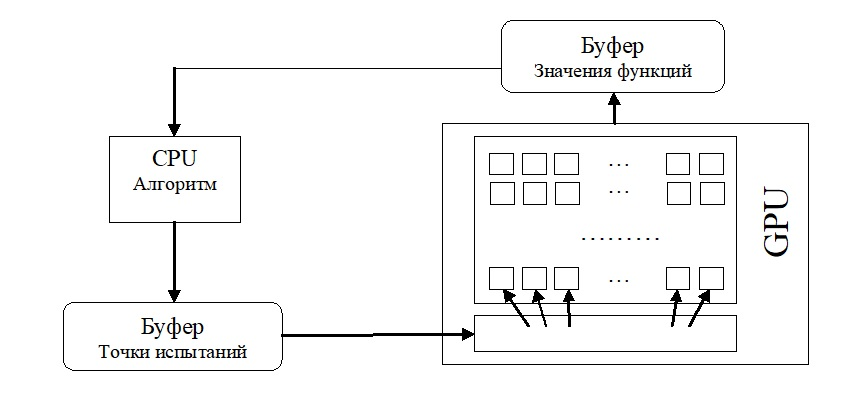
\includegraphics[width=1.0\textwidth] {fig2.jpg}
    \caption{Схема информационных обменов в GPU-алгоритме}
    \label{fig:2}
\end{figure}

Общая схема организации вычислений с использованием GPU приведена на Fig.  \ref{fig:2}. В соответствии с данной схемой на CPU выполняются шаг 1 – 6 параллельного алгоритма глобального поиска. Координаты \textit{p} точек испытаний, вычисленные на шаге 7 алгоритма, накапливаются в промежуточном буфере, а затем передаются на графический процессор. На GPU происходит вычисление значений функции в этих точках, после чего результаты испытаний (снова через промежуточный буфер) передаются на CPU.




\section{Results of experiments}

Let us compare proposed MIPIA with a genetic algorithm for solving the mixed-integer global optimization problems implemented in Matlab Global Optimization Toolbox \cite{Matlab}. In Table 
\ref{tab:1}, the numbers of trials required for solving the known test mixed-integer 
problems by these methods are presented. For both methods, the same accuracy of search $10^{-2}$ were used. All numerical experiments were conducted on a 
computer with Intel Core i5-7300 2.5 GHz processor and 8 Gb RAM under MS Windows 10. The 
results of experiments have demonstrated the advantage of MIPIA in the number 
of iterations as well as in the execution time.

\begin{table}
	\caption{Comparison of MIPIA and GA}
	\label{tab:1}
	\center
	\begin{tabular}{cccccc}
		\hline\noalign{\smallskip}
	\multirow{2}{*}{Test problem}	 & \multicolumn{2}{c}{ GA } & & \multicolumn{2}{c}{MIGSA} \\
		\noalign{\smallskip} \cline{2-3} \cline{5-6} \noalign{\smallskip}
		 & $k$ & $t$ & & $k$ & $t$  \\
		\noalign{\smallskip} \hline \noalign{\smallskip}
		 Problem 2 \cite{Floudas}&	481 &	0.0601 & &	417 &	0.04 \\
%		 Problem 3 \cite{Floudas}& 	1821 &	0.1130 & & 3324 &	0.107 \\
		 Problem 6 \cite{Floudas}&	641 &	0.0510 & &	118 &	0.001 \\
		 Problem 1 \cite{Deep}   &	481 &	0.1378 & &	66 &	0.0007 \\
		 Problem 2 \cite{Deep}   &	481 &	0.0473 & &	57 &	0.0006 \\
		 Problem 7 \cite{Deep}   &	841 &	0.0736 & & 372	 &	0.017 \\
		\noalign{\smallskip}\hline
	\end{tabular}
\end{table}

%In order to demonstrate the reliability of the MIGSA method, we have solved two series of 100 multiextremal mixed-integer problems each constructed on the basis of modified problems of \textit{Simple} and \textit{Hard} classes generated by GKLS generator. 

Известным генератором тестовых задач непрерывной многоэкстремальной оптимизации является GKLS-генератор \cite{Gaviano}. Он позволяет генерировать functions of arbitrary dimensionality with known properties (the number of local minima, the size of their domains of attraction, the global minimizer, etc.).  
This generator of multiextremal functions is often used for the investigations of the global optimization algorithms~ 
\cite{Paulavicius2014,SergeyevKvasov2015,Lebedev2015,Gergel2015}.
%Линии уровня какой-нибудь задачи GKLS? C точками испытаний?

В проведенных экспериментах GKLS-генератор использовался как основа для построения mixed-integer problems. Правила, позволяющие генерировать тестовые задачи подобного вида, заключаются в следующем.

\begin{enumerate}
	\item С помощью генератора GKLS порождается непрерывная многоэкстремальная функция $\varphi(y), \; y\in D, \; D = \left\{ a_j\leq y_j\leq b_j, 1\leq j \leq N \right\}$. Глобальный минимум данной функции достигается в известной точке $y'=(y'_1,...,y'_N)$ и равен $\varphi'=\varphi(y')=-1$.
	\item Генерируется concave mixed-integer function 
	\[
			\mu(y,u) = -2 \left[ \sum_{j=1}^N \left( \frac{y_j - y'_j}{b_j-a_j} \right)^2 + \sum_{j=1}^M \left( \frac{u_j - b_j}{b_j-a_j} \right)^2 \right].
	\]
	где $y\in D = \left\{ a_j\leq y_j\leq b_j, 1\leq j \leq N \right\} \subset R^N$, a $u\in U = = \left\{ a_j\leq u_j\leq b_j, 1\leq j \leq M \right\} \subset Z^N$; т.е. данная функция имеет $N$ непрерывных и $M$ дискретных параметров и достигает минимального значения в точке $(y',b)$.
	\item Вычисляется коэффициент 
	\[
	C = 4 - \min_{y,u} \left\{ \mu(y,u) \right\}, \; y\in D, u \in U.
	\]
	Очевидно, что минимум вогнутой функции $\mu(y,u)$ в одной из угловых точек области поиска, поэтому при размерности задачи порядка 10 его вычисление может быть выполнено методом перебора.
	\item Формируется многоэкстремальная mixed-integer function 
	\[
	f(y,u) = \left(\varphi(y) + \sum_{j=1}^M{u_j}\right)\left(C + \mu(y,u)\right).
	\]
	По построению $f(y,u)$  будет принимать минимальное значение в точке $(y',b)$.
	
\end{enumerate}


In the problems generated in our experiments, there were 5 integer  and 6 continuous parameters. Дискретные параметры имеют по 4 значения, таким образом имеем \textit{S} = 1024 возможных значения. С помощью GKLS-генератора создано 100 шестимерных задач, которые были преобразованы в смешанные 11-ти мерные задачи. The accuracy of the search was equal to $10^{-2}$.   
Computational experiments were carried out on Lobachevsky supercomputer. The node of 
supercomputer included two Intel Sandy Bridge E5-2660 2.2 GHz CPUs and 64 Gb RAM. The 
CPU had 8 cores, i.e. each node had a total of 16 cores and two NVIDIA Kepler K20Х GPUs.



В Table \ref{tab:2} приведены результаты экспериментов на CPU с использованием OpenMP. Использовалось 1, 8 и 16 потоков. Приведено среднее число итераций требуемое для решения задачи, среднее время решения (в секундах) и ускорение по времени по отношению к последовательному запуску. За одну итерацию проводилось столько же испытаний сколько использовалось потоков.

\begin{table}
	\caption{Результаты экспериментов на CPU}
	\label{tab:2}
	\center
	\begin{tabular}{cccccc}
		\hline\noalign{\smallskip}
        
		Число потоков & \textit{p} = 1 & \textit{p} = 8 & \textit{p} = 16 \\
	\noalign{\smallskip} \hline \noalign{\smallskip}

		Среднее число итераций  & 3 221 023,4 & 512 314,2 & 209 237,0 \\
		Среднее время решения & 5 520,3 & 1 253,5 & 717,3 \\
		Ускорение по отношению к одному потоку & 1,0 & 4,4 & 7,7 \\
		\noalign{\smallskip}\hline
	\end{tabular}
\end{table}


Как видно из Table \ref{tab:2} , наблюдается почти линейное ускорение по итерациям и значительное ускорение по времени решения задачи. В среднем при последовательном решение задачи требовалось 1,5 часа.

В Table \ref{tab:3} приведены результаты экспериментов на GPU с использованием CUDA. Использовалось 256, 512 и 1024 нитей. Приведено среднее число итераций требуемое для решения задачи, среднее время решения (в секундах) и ускорение по времени по отношению к полной загрузке CPU на узле кластера. За одну итерации проводилось столько же испытаний сколько использовалось нитей.

\begin{table}
	\caption{Результаты экспериментов на GPU}
	\label{tab:3}
	\center
	\begin{tabular}{cccccc}
		\hline\noalign{\smallskip}
        
		Число нитей & \textit{p} = 256 & \textit{p} = 512 & \textit{p} = 1024 \\
	\noalign{\smallskip} \hline \noalign{\smallskip}

		Среднее число итераций  & 1 522,3 & 919,8 & 412,6 \\
		среднее время решения & 33,6 & 31,2 & 30,2 \\
		Ускорение по отношению к полной загрузке ЦПУ & 21,4 & 23,0 & 23,7 \\

		\noalign{\smallskip}\hline
	\end{tabular}
\end{table}

Наблюдается значительное ускорение как по числу итераций, так и по времени. В среднем решение задачи (при 1024 нитях) потребовало 30 секунд. Таким образом, ускорение по отношению к последовательному запуску составило 182.

%All problems of the series have been solved successfully and for solving the problems based on the \textit{Simple} class 11988 trials in average were required whereas for solving the problems based on the \textit{Hard} class 24750 trials were required.

\section{Conclusion}

Заключение 

%\textbf{Acknowledgments}. This study was supported by the Russian Science Foundation, project No 16-11-10150.

\begin{thebibliography}{10}

\bibitem{Burer}
Burer, S., Letchford, A.N.: Non-convex mixed-integer nonlinear programming: A survey. Surveys in Operations Research and Management Science \textbf{17}, 97--106 (2012) 

\bibitem{Boukouvala}
Boukouvala, F., Misener, R., Floudas, C.A.: Global optimization advances in Mixed-Integer Nonlinear Programming, MINLP, and Constrained Derivative-Free Optimization, CDFO. European J. Oper. Res. \textbf{252}, 701--727 (2016) 

\bibitem{Strongin2000}
Strongin, R.G., Sergeyev, Y.D.: Global optimization with non-convex constraints. Sequential and parallel algorithms. Kluwer Academic Publishers, Dordrecht (2000) %; DOI: 10.1007/978-1-4615-4677-1

\bibitem{Strongin2013}
Sergeyev, Ya.D., Strongin, R.G., Lera, D.: Introduction to global optimization exploiting space-filling curves. Springer (2013) %;  DOI: 10.1007/978-1-4614-8042-6

\bibitem{Floudas}
Floudas, C.A., Pardalos, P.M.:  Handbook of test problems in local and global optimization. Springer (1999)  %; DOI: 10.1007/978-1-4757-3040-1

\bibitem{Matlab}
https://www.mathworks.com/help/gads/mixed-integer-optimization.html

\bibitem{Deep}
Deep, K., Singh, K. P., Kansal, M.L., Mohan, C.: A real coded genetic algorithm for solving integer and mixed integer optimization problems. Appl. Math. Comput. \textbf{212}(2), 505--518 (2009)

\bibitem{Gaviano} Gaviano, M., Kvasov, D.E, Lera, D., and Sergeyev, Ya.D.: Software for generation of classes of test functions with known local and global minima for global optimization. ACM Transactions on Mathematical Software \textbf{29}(4), 469--480 (2003)

\bibitem{Paulavicius2014} 
Paulavi\v{c}ius, R., Sergeyev, Y., Kvasov, D., \v{Z}ilinskas, J.: Globally-biased DISIMPL algorithm for expensive global optimization. J. Glob. Optim. \textbf{59}(2-3), 545--567 (2014)

\bibitem{SergeyevKvasov2015} 
Sergeyev, Y.D., Kvasov, D.E.: A deterministic global optimization using smooth diagonal auxiliary functions. Commun. Nonlinear. Sci. Numer. Simulat. \textbf{21}(1-3), 99--111 (2015)

\bibitem{Lebedev2015}
Lebedev, I., Gergel, V.: Heterogeneous parallel computations for solving global optimization problems. Procedia Computer Science \textbf{66}, 53--62 (2015)

\bibitem{Gergel2015}
Gergel, V., Sidorov, S.: A two-level parallel global search algorithm for solution of computationally intensive multiextremal optimization problems. Lecture Notes in Computer Science  \textbf{9251}, 505--515 (2015)


\end{thebibliography}


\end{document}
______________________________________________________________________
